\documentclass[12pt]{article}
\usepackage[english,greek]{babel}
\usepackage[utf8]{inputenc}
\usepackage{enumitem}
\usepackage{titling}
\usepackage{amsmath}
\usepackage{graphicx}
\usepackage{pgfplots}
\setlength{\droptitle}{-12em} 

\title{Ανάλυση Σχεδίαση Συστημάτων Λογισμικού}
%\vspace{-30pt}
\author{\textbf{Εργασία 2017-2018} \\Νέμανια Νέντιτς \\ Α.Μ. 111520140124 \\ Κωνσταντίνος Στεφανίδης - Βοζίκης \\ Α.Μ. 1115201400192}
\date{}
\begin{document}
\maketitle
\section*{Αντικειμενοστραφής Ανάλυση και Σχεδιασμός}
\begin{enumerate}
\item
Οι μη λειτουργικές απαιτήσεις του συστήματος είναι:
\begin{itemize}
\item
Λήψη αντιγράφων (\textlatin{back up}) κάθε ώρα
\item
Λειτουργία του συστήματος 24 ώρες το 24ώρο
\end{itemize}
\item
\begin{tabular}{|l|l|}
\hline
'Εννοια & Περιγραφή \\
\hline
Διδάσκων & Υπάλληλος του πανεπιστημίου που διδάσκει \\
\hline
ΕΔΙΠ & Διδάσκων πλήρους απασχόλησης \\
\hline
Συμβασιούχος & Διδάσκων με σύμβαση συγκεκριμένου χρόνου \\
\hline
Συμβόλαιο & Συμφωνία μεταξύ του πανεπιστημίου και ενός συμβασιούχου \\
\hline
Άδεια & Χρονικό διάστημα που ένας μόνιμος διδάσκων δεν δουλέυει \\ 
\hline
Τρόπος πληρωμής & Τρόπος με τον οποίο ένας διδάσκων λαμβάνει την αμοιβή \\ 
& του από το πανεπιστήμιο \\
\hline
Ειδοποίηση πληρωμής & Τρόπος με τον οποίο ένας συμβασιούχος ενημερώνεται για \\
 & τα χρήματα που εισπράττει από το πανεπιστήμιο \\
\hline
Πληρωμή & Αμοιβή του πανεπιστημίου προς έναν διδάσκοντα για \\ 
& την εργασία του \\ 
\hline
Χρονοκάρτα & Κατάσταση στην οποία ένας συμβασιούχος διδάσκων \\
 & υποβάλλει στο σύστημα για να μετρηθούν οι μέρες \\
 &  και ώρες διδασκαλίας του. \\
\hline
\end{tabular}

\item
Το διάγραμμα περιπτώσεων χρήσης είναι το παρακάτω:\\
\begin{center}
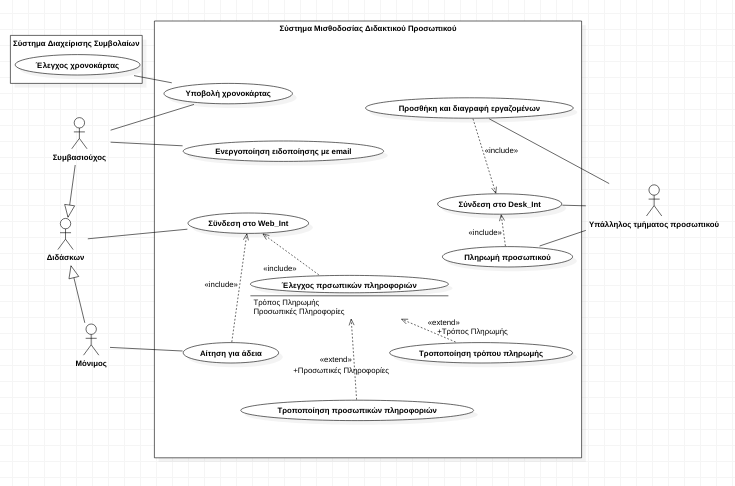
\includegraphics[scale=0.6]{use_case}
\end{center}

\item
Το διάγραμμα κλάσεων είναι το παρακάτω:\\
\begin{center}
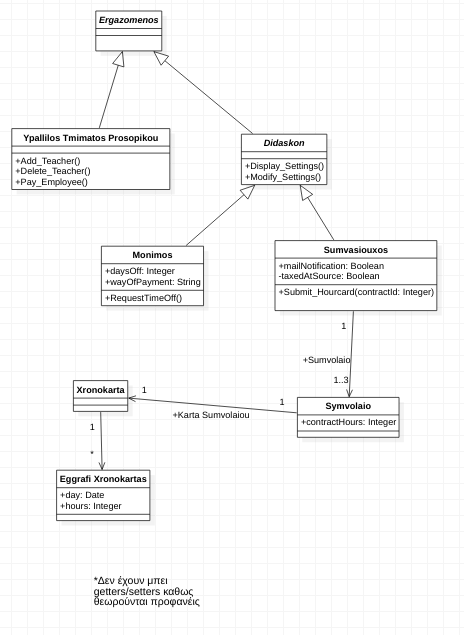
\includegraphics[scale=0.6]{class_diag}
\end{center}

\item

\item
Το διάγραμμα δραστηριοτήτων είναι το παρακάτω:\\
\begin{center}
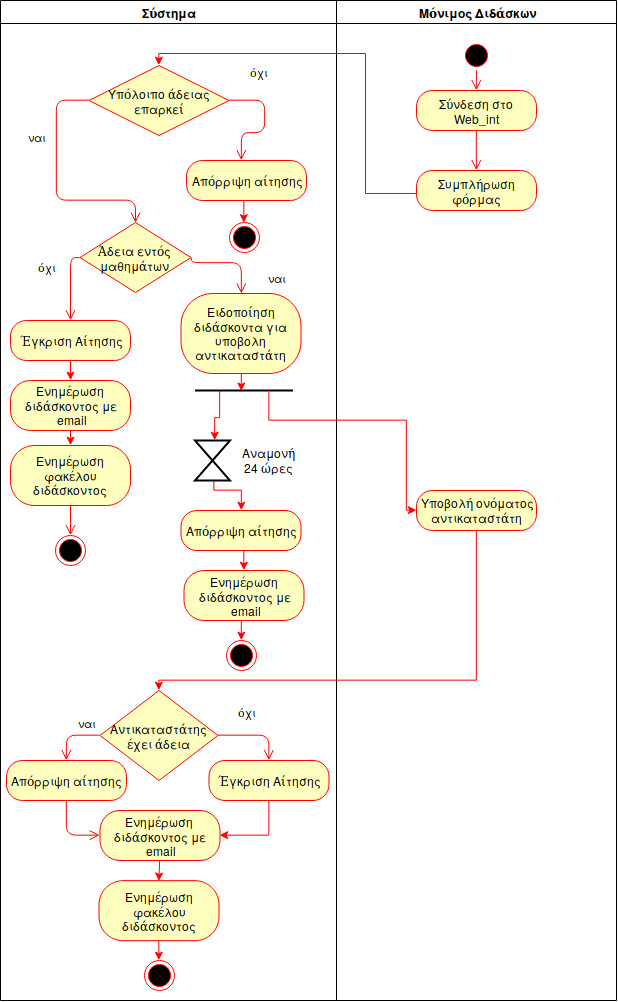
\includegraphics[scale=0.5]{activity}
\end{center}

\item
Το διάγραμμα καταστάσεων είναι το παρακάτω:\\
\begin{center}
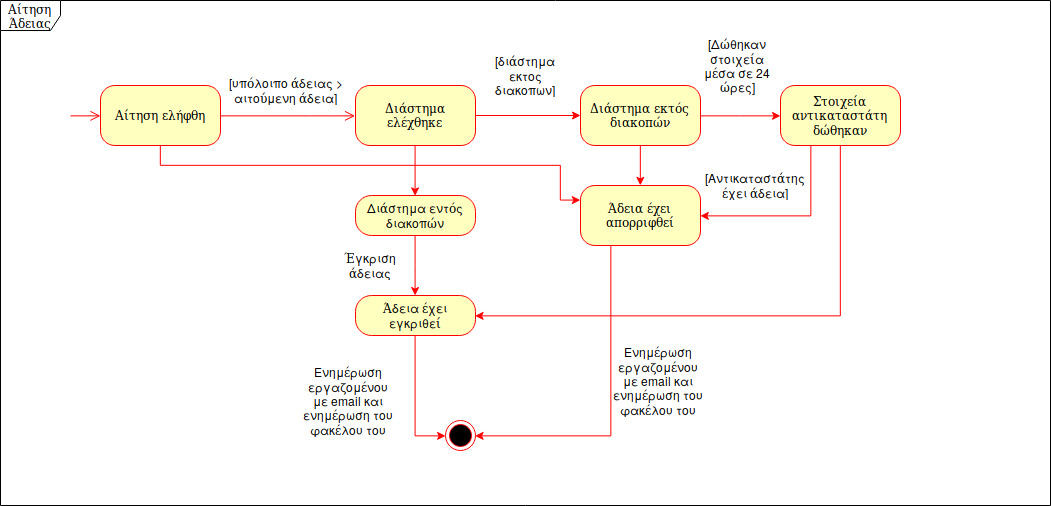
\includegraphics[scale=0.4]{state_diag}
\end{center}

\item

\item
\end{enumerate}


\section*{Δομημένη Ανάλυση}

\section*{Δομημένος Σχεδιασμός}


\end{document}